% Class
\documentclass[11pt,a4paper]{article}

% Codage
\usepackage[utf8]{inputenc}
\usepackage[T1]{fontenc}
\usepackage{siunitx}
\usepackage{indentfirst}

% Langue
\usepackage[english]{babel}

% Supplément
\usepackage{amsmath,amsfonts,amssymb}
\usepackage{verbatim} % pour faire des commentaires avec \begin{comment}...
\usepackage{float} % pour positioner un image exacetement où on veut
\usepackage
  [separate-uncertainty = true,
  multi-part-units = repeat]
  {siunitx} % Exemple \SI{0}{\kg \cdot \m^{-3}}

% Images
\usepackage[pdftex]{graphicx}
\usepackage{graphics}
\usepackage{subcaption} % pour positioner des figures côte à côte
\usepackage{wrapfig}

% pour l'inclusion de liens dans le document 
\usepackage[colorlinks,bookmarks=false,linkcolor=blue,urlcolor=blue]{hyperref}

\usepackage{amsmath}
\usepackage{listings}
\usepackage{xcolor}


% la mise en page
\usepackage{geometry}
\paperheight=297mm
\paperwidth=210mm

\pagestyle{plain}

\definecolor{codegreen}{rgb}{0,0.6,0}
\definecolor{codegray}{rgb}{0.5,0.5,0.5}
\definecolor{codepurple}{rgb}{0.58,0,0.82}
\definecolor{backcolour}{rgb}{0.95,0.95,0.92}

\lstdefinestyle{mystyle}{
    backgroundcolor=\color{backcolour},   
    commentstyle=\color{codegreen},
    keywordstyle=\color{magenta},
    numberstyle=\tiny\color{codegray},
    stringstyle=\color{codepurple},
    basicstyle=\ttfamily\footnotesize,
    breakatwhitespace=false,         
    breaklines=true,                 
    captionpos=b,                    
    keepspaces=true,                 
    numbers=left,                    
    numbersep=5pt,                  
    showspaces=false,                
    showstringspaces=false,
    showtabs=false,                  
    tabsize=2
}

\lstset{style=mystyle}



% nouvelles commandes LaTeX, utilis\'ees comme abreviations utiles
\newcommand{\mail}[1]{{\href{mailto:#1}{#1}}}
\newcommand{\ftplink}[1]{{\href{ftp://#1}{#1}}}

%%%%%%%%%%%%%%%%%%%%%%%%%%%%%%%%%%%%%%%%%%%%%%%%%%%%%%%%
\begin{document}


% Le titre, l'auteur et la date
\title{Physics of Nuclear Reactor - Numerical Exercises}
\author{Noah Rotunno\\  % \\ pour fin de ligne
}
\date{\today}
\maketitle
%%%%%%%%%%%%%%%%%%%%%%%%%%%%%%%%%%%%%%%%%%%%%%%%%%%%%%%%

% *******************************************************************************
% *** Exercice 1 ****************************************************************
% *******************************************************************************

\newpage

% Small precisions
To run an exercice, open CMD and run the main file. The scripts that run a simulation is always named as main : \\
\begin{lstlisting}
preject_path/exercice_i> python main.py
\end{lstlisting}

Some scripts can create other files:
\begin{enumerate}
	\item pdf : Figure used in the report
	\item npy : file to save a numpy array. This is used for saving data for big convergence study.
\end{enumerate}

WARNING : In certain convergence studies, the plots generated by the Python script differ from those presented in the report. This discrepancy arises because the report plots were produced using a higher number of simulations to obtain better plots. However, for efficiency and to reduce computation time, the number of simulations was lowered in the submission scripts.

\section{Exercice \#1 - Modeling a planar source of neutrons}

\subsection{Question \#1}
\begin{figure}[h]
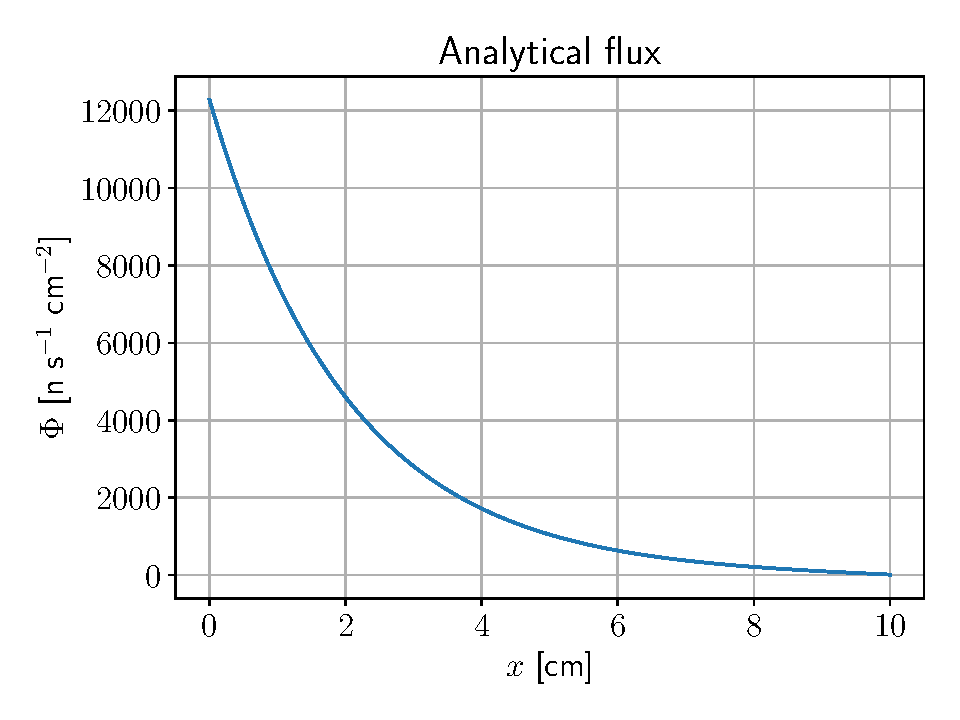
\includegraphics[width=10cm]{fig/Ex1_Analytical.pdf}
\centering
\caption{Analytical Solution for the neutron flux as a function of depth.}
\end{figure}
Flux values at the following locations (4 significant digits):\\
Flux value at $x_0$: 13.5896 n cm$^{-2}$ s$^{-1}$ \\
Flux value at $0$: 12276.8979 n cm$^{-2}$ s$^{-1}$ \\

\subsection{Question \#2}

Relationship between $\mathrm{\Phi}_i,\ \mathrm{\Phi}_{i+1},\ \mathrm{\Phi}_{i-1}$ at any point within the material:
\begin{equation}
    A \Phi_i + B \Phi_{i-1} +C \Phi_{i+1} = D
\end{equation}

Coefficients of the matrix A (4 significant digits), for a mesh size of 0.1cm:\\
Coef $A_{i,i}$: -16.6037 \\
Coef $A_{i-1,i}$: 8.2919 \\
Coef $A_{i+1,i}$: 8.2919 \\

Relationship between $\mathrm{\Phi}_i,\ \mathrm{\Phi}_{i-1},\ \mathrm{\Phi}_{i+1}$, \\
at the source:
\begin{equation}
    A \Phi_1 + B \Phi_{2} = C
\end{equation}
at the RHS of the problem:
\begin{equation}
    A \Phi_n + B \Phi_{n-1} = C
\end{equation}
Associated coefficients of the matrix A (4 significant digits), for a mesh size of 0.1cm:
at the source: \\
Coef $A_{1,i}$: -8.3119 \\
Coef $A_{2,i}$: 8.2919 \\
at the RHS: \\
Coef $A_{n-1,i}$: 8.2919 \\
Coef $A_{n,i}$: -12.1536 \\

\subsection{Question \#3}

Flux values from the numerical solver at the following locations (4 significant digits):\\
Flux value at $x_0$: 13.6244 \\
Flux value at $0$: 12280.5980 \\

Add two sentences describing what you see in Figure \ref{err} and a possible explanation :
The error decrease as the mech increase, meaning that the simulation converge. The order of convergence has been evaluated to $\sim  1$. 

\begin{figure}[H]
	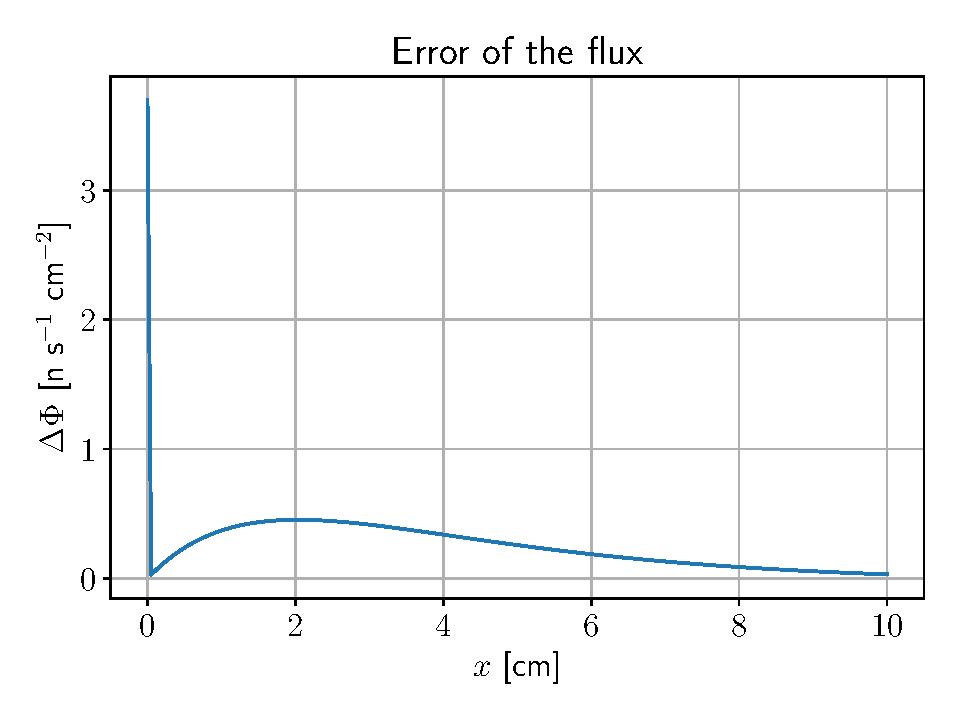
\includegraphics[width=10cm]{fig/Ex1_Error.pdf}
	\centering
	\caption{Distance between the solutions at each mesh point for a mesh size of 0.1 cm.}
\end{figure}

\begin{figure}[H]
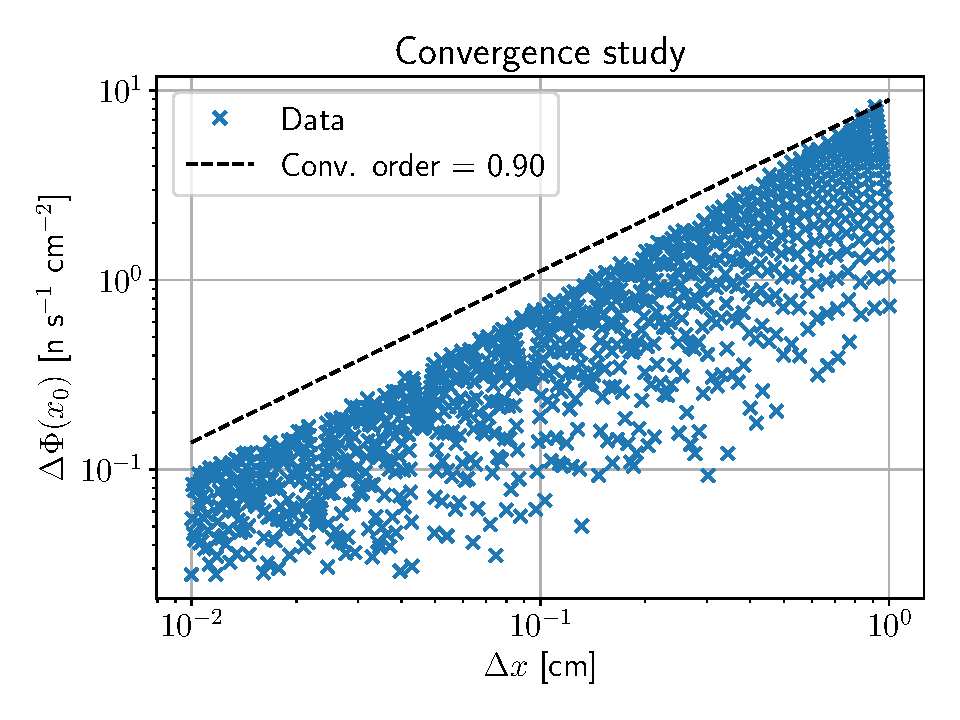
\includegraphics[width=10cm]{fig/Ex1_conv_N1000.pdf}
\centering
\caption{Evolution with mesh size of the absolute error of $\Phi(x_0)$.}
\label{err}
\end{figure}





% *******************************************************************************
% *** Exercice 2 ****************************************************************
% *******************************************************************************

\newpage
\section{Exercice \#2 - Modeling a planar reactor (1 group)}

\subsection{Question \#1}
\begin{figure}[H]
	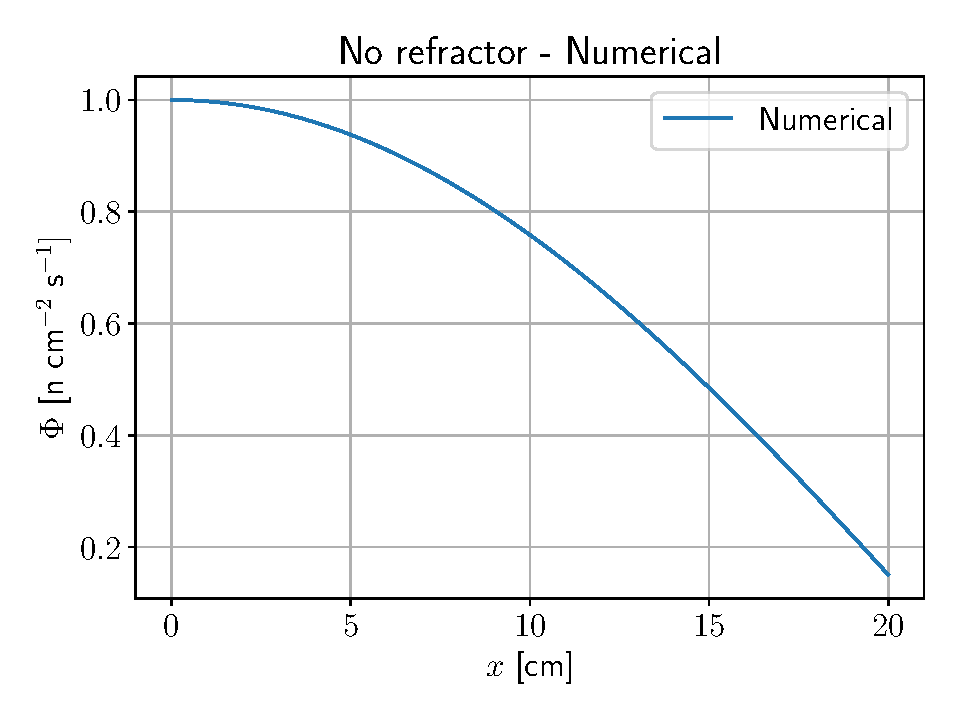
\includegraphics[width=10cm]{fig/Ex2_Q1.pdf}
	\centering
	\caption{Flux in the bare reactor for a mesh size of 0.1 cm.}
\end{figure}
Numerical solution for the bare system \\
keff (scientific format with 5 significant digits): 0.97305 \\
Net current at the core boundary (scientific format with 5 significant digits): 0.075436 \\

\subsection{Question \#2}
\begin{figure}[H]
	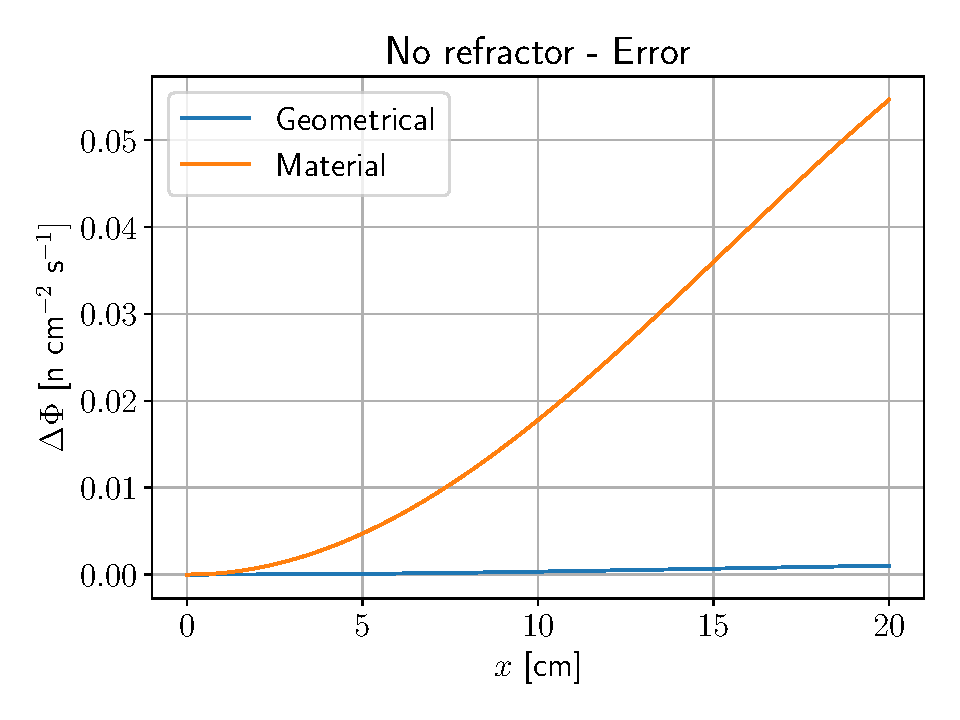
\includegraphics[width=10cm]{fig/Ex2_Q2.pdf}
	\centering
	\caption{Distance between the solutions at each mesh point for a mesh size of 0.1 cm.}
\end{figure}
Analytical solution for the bare system \\
keff (scientific format with 5 significant digits): 0.97356 \\
Net current at the core boundary (scientific format with 5 significant digits): 0.075367 \\

\subsection{Question \#3}
Numerical solution for the reflected system \\
keff (scientific format with 5 significant digits): 1.12038 \\
Net current at the core boundary (scientific format with 5 significant digits): -0.054402 \\
\begin{figure}[H]
	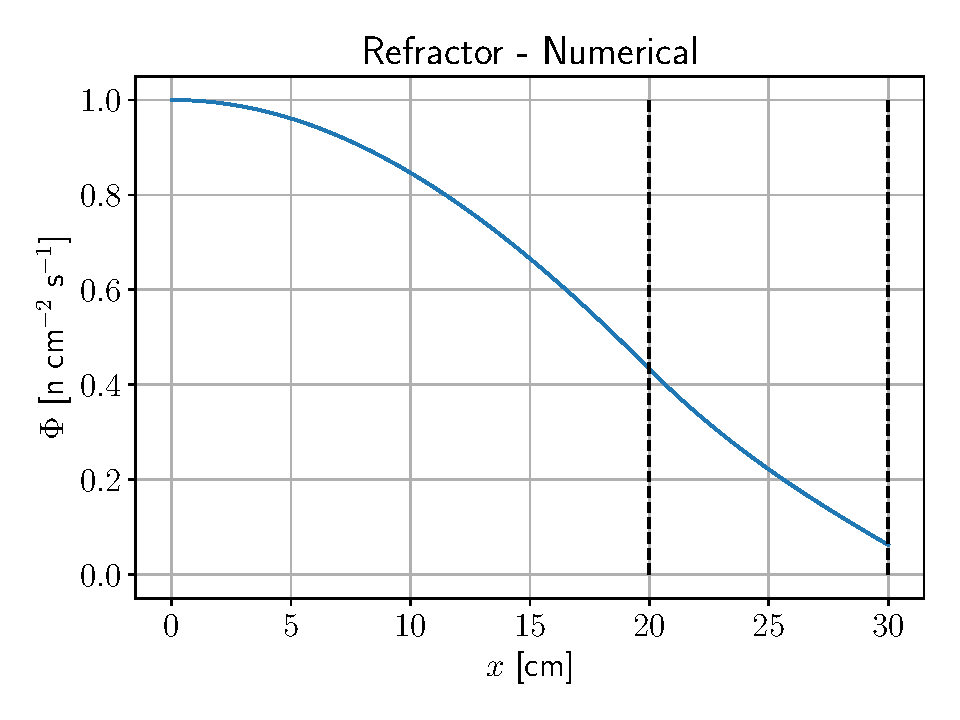
\includegraphics[width=10cm]{fig/Ex2_Q3.pdf}
	\centering
	\caption{Flux in the reflected reactor for a mesh size of 0.1 cm.}
\end{figure}





% *******************************************************************************
% *** Exercice 3 ****************************************************************
% *******************************************************************************

\newpage
\section{Exercice \#3 - Modeling a planar reactor (2 groups)}

\subsection{Question \#1 Numerical formulation}

Relationship between $\mathrm{\Phi}_i,\ \mathrm{\Phi}_{i+1},\ \mathrm{\Phi}_{i-1}$ for group g at any point within the material:
\begin{equation}
	A \Phi_i + B \Phi_{i-1} +C \Phi_{i+1} = D
\end{equation}

Expression of the source term for the fast and thermal energy group:
\begin{equation}
	\begin{split}
		b_1 &= \nu \Sigma_{f1} \Phi_1 + \nu \Sigma_{f2} \Phi_2 \\
		b_2 &= \Sigma_{s1 \rightarrow 2} \Phi_1
	\end{split}
	\end{equation}

\subsection{Question \#2 Analytical solution for the bare system}
\begin{equation}
	k_{eff}= \frac{\nu \Sigma_{f1} (B^2D_2 + \Sigma_{t2}) + \Sigma_{s}^{1 \rightarrow 2} \nu \Sigma_{f2}}{(B^2D_1 + \Sigma_{t1})(B^2D_2 + \Sigma_{t2}) - \Sigma_s^{1 \rightarrow 2} \Sigma_s^{2 \rightarrow 1}}
\end{equation}


keff (scientific format with 5 significant digits): 1.08440 \\

\subsection{Question \#3 Numerical solution of the bare homogeneous reactor}



keff (scientific format with 5 significant digits): 1.08677 \\

fast buckling (scientific format with 5 significant digits): 0.030229 \\

thermal buckling (scientific format with 5 significant digits): 0.030348 \\

\begin{figure}[H]
	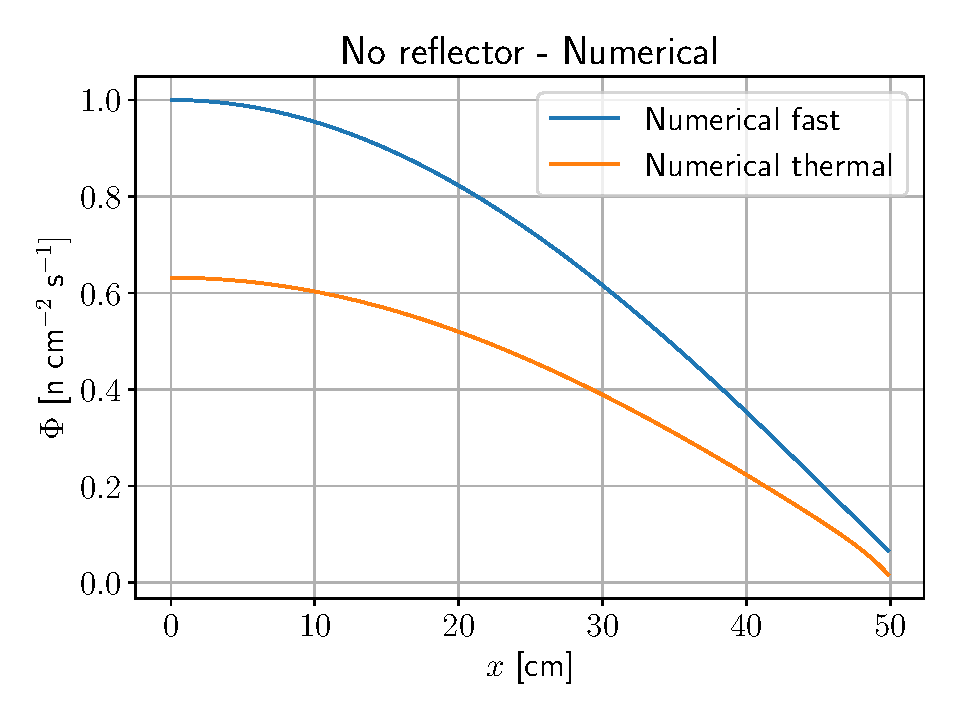
\includegraphics[width=10cm]{fig/Ex3_BarePhi.pdf}
	\centering
	\caption{Fast and thermal fluxes in the bare reactor for a mesh size of 0.1 cm.}
\end{figure}

\subsection{Question \#4}
\begin{figure}[H]
	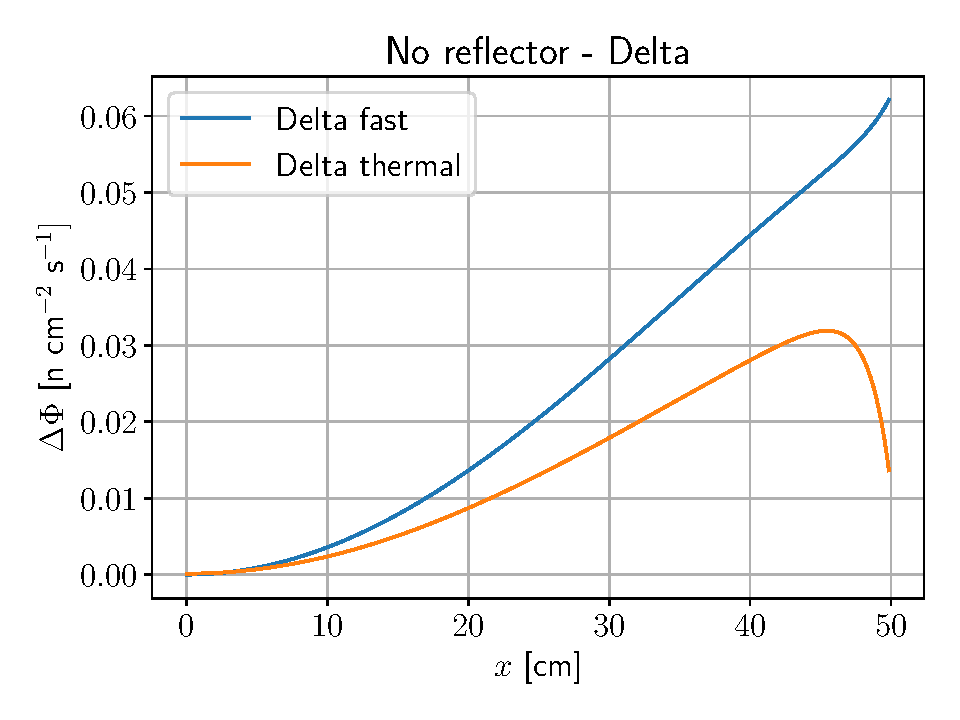
\includegraphics[width=10cm]{fig/Ex3_BareDelta.pdf}
	\centering
	\caption{Difference between numerical and analytical solutions for the fast and thermal fluxes in the bare reactor for a mesh size of 0.1 cm.}
\end{figure}

\subsection{Question \#5 Numerical solution of the reflected reactor}


keff (scientific format with 5 significant digits): 1.09199 \\

fast net current (scientific format with 5 significant digits) at the core/reflector interface: -0.039511 \\

thermal net current (scientific format with 5 significant digits) at the core/reflector interface: 0.0058747 \\

\begin{figure}[H]
	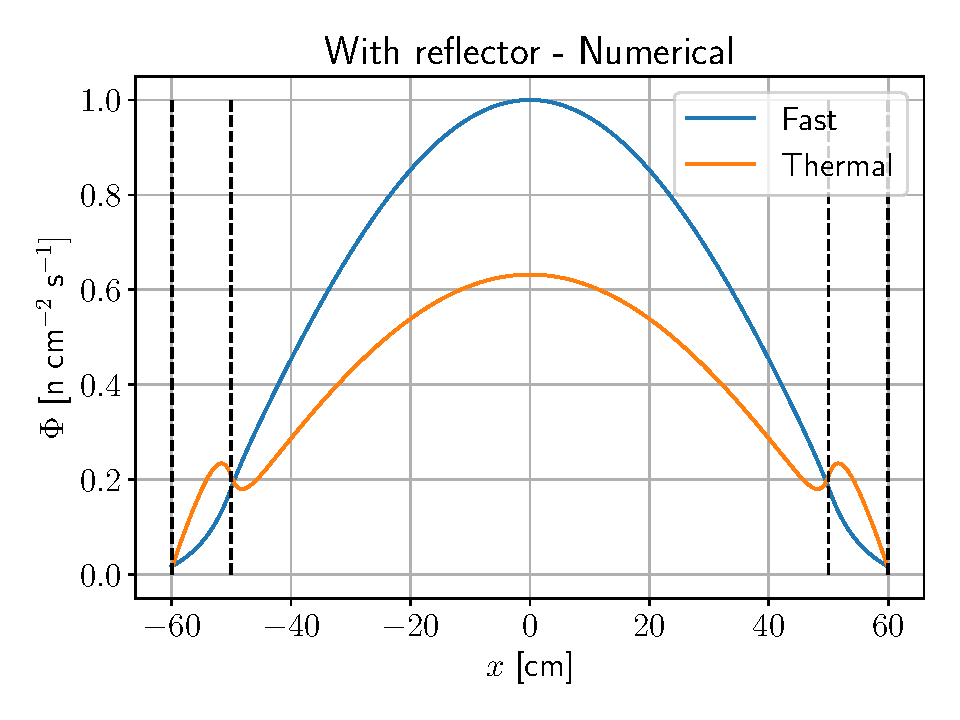
\includegraphics[width=10cm]{fig/Ex3_ReflectorH0.pdf}
	\centering
	\caption{Fast and thermal fundamental fluxes in the reflected reactor for a mesh size of 0.1 cm.}
\end{figure}

\begin{figure}[H]
	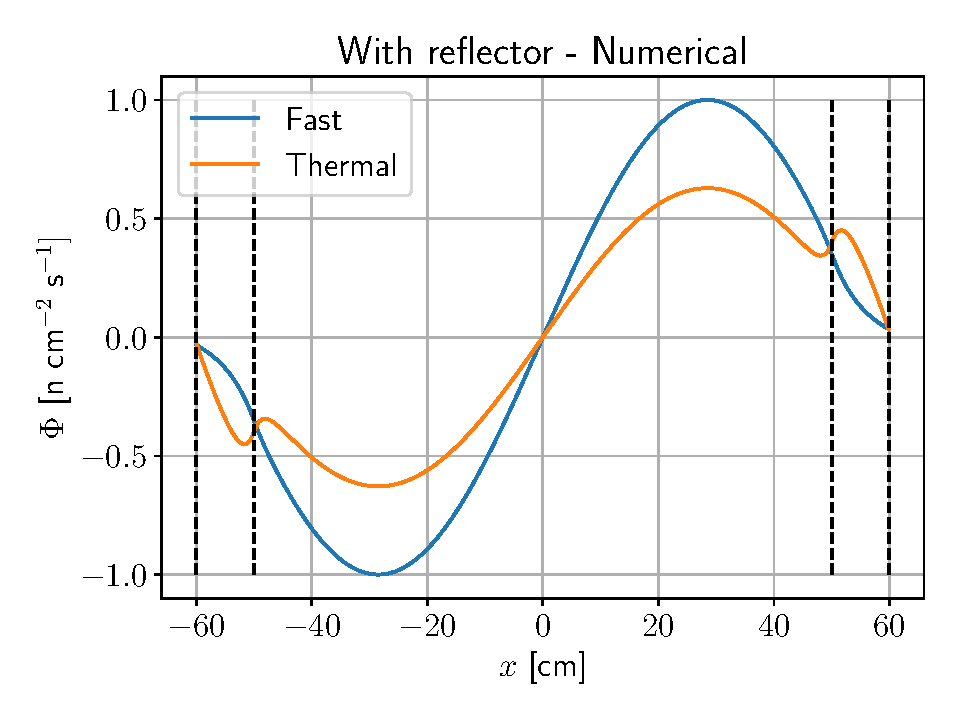
\includegraphics[width=10cm]{fig/Ex3_ReflectorH1.pdf}
	\centering
	\caption{Fast and thermal first harmonic of the fluxes in the reflected reactor for a mesh size of 0.1 cm.}
\end{figure}

first harmonic eigenvalue (scientific format with 5 significant digits): 1.02113 \\





% *******************************************************************************
% *** Exercice 4 ****************************************************************
% *******************************************************************************

\newpage
\section{Exercice \#4 - Modeling a more realistic planar reactor in two groups}

\subsection{Question \#1 Initial Loading Pattern}

keff (scientific format with 5 significant digits): 1.21882 \\

peak power (scientific format with 5 significant digits): $7.37503 \cdot 10^5$ W \\

fast flux at the core boundary (scientific format with 5 significant digits): $1.87308 \cdot 10^{15}$ n cm$^{-2}$ s$^{-1}$\\

\begin{figure}[h]
	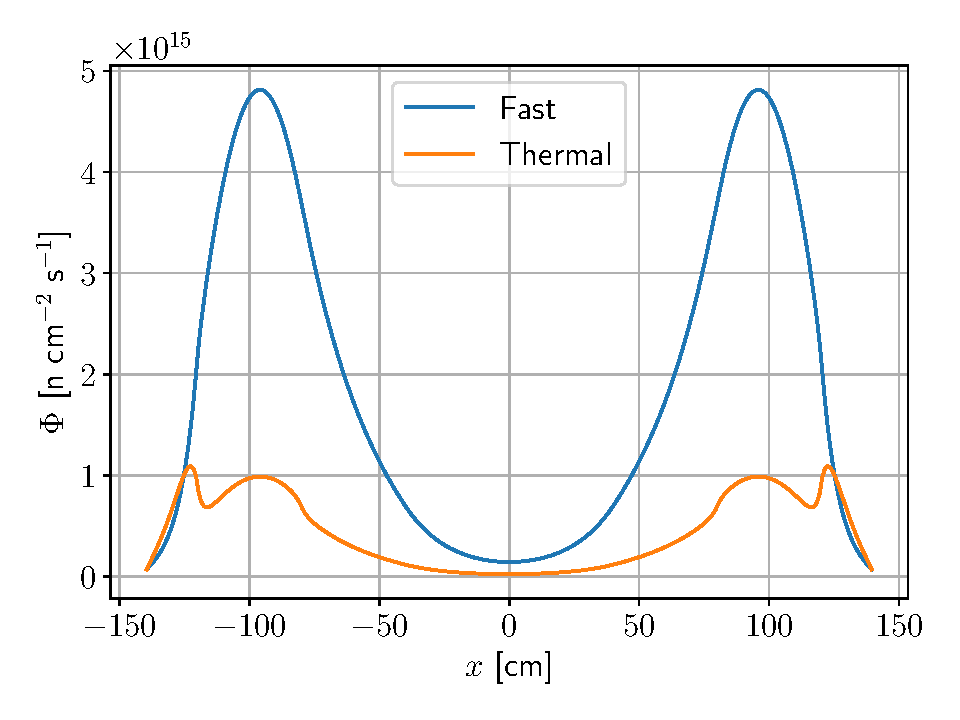
\includegraphics[width=10cm]{fig/Ex4_Flux.pdf}
	\centering
	\caption{Normalized fast and thermal fluxes}
\end{figure}

\begin{figure}[h]
	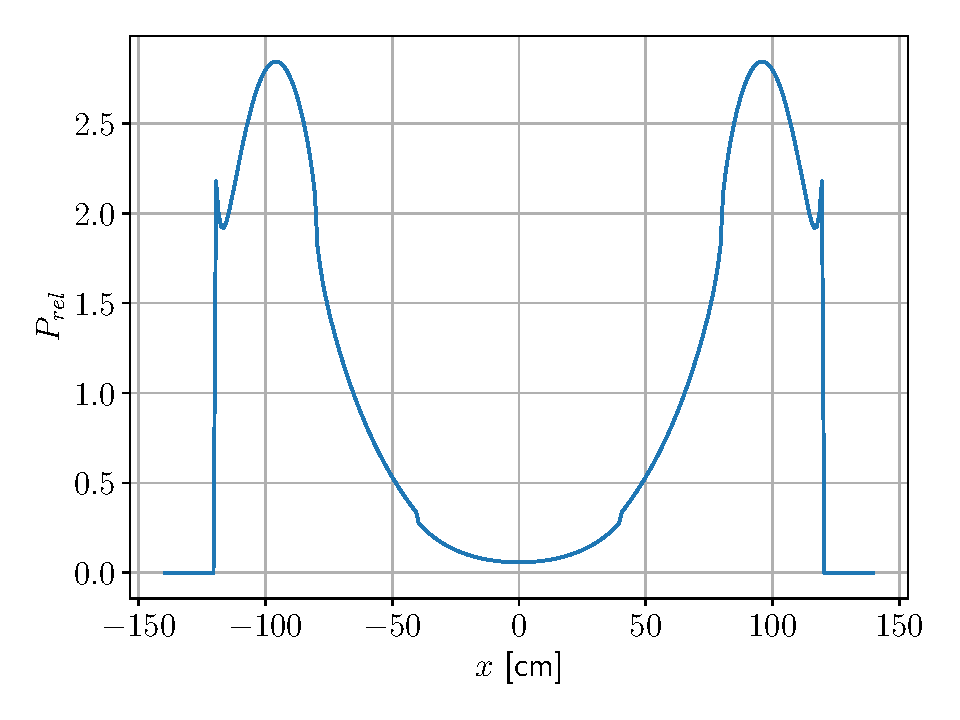
\includegraphics[width=10cm]{fig/Ex4_Power.pdf}
	\centering
	\caption{Relative power distribution}
\end{figure}

Explanation of the main features of the power distribution: The newest batch are placed at the right boundray, meaning that more fission product are present in the middle of the reactor. This mean that the neutrons are more absorbed in the middle, leading to a greater flux at the boundary. Moreover, the newest batch create more fission meaning more power and the reflector reflect a part of the neutrons at the boundary leading to a small increase in the power at the boundary. \\


\subsection{Question \#2 Optimized Loading Pattern}

\begin{table}[H]
	\centering
	\begin{tabular}{|c|c|c|c|c|c|c|}
		\hline
		2& 1& 2& 3& 1& 3& 4\\
		\hline
	\end{tabular}
	\caption{Loading pattern from the core center (left to right)}
\end{table}

keff (scientific format with 5 significant digits): 1.19399 \\

peak power (scientific format with 2 significant digits): $6.53340 \cdot 10^{5}$ W\\

fast flux at the core boundary (scientific format with 2 significant digits):$6.28 \cdot 10^{13}$ n cm$^{-2}$ s$^{-1}$\\

\begin{figure}[H]
	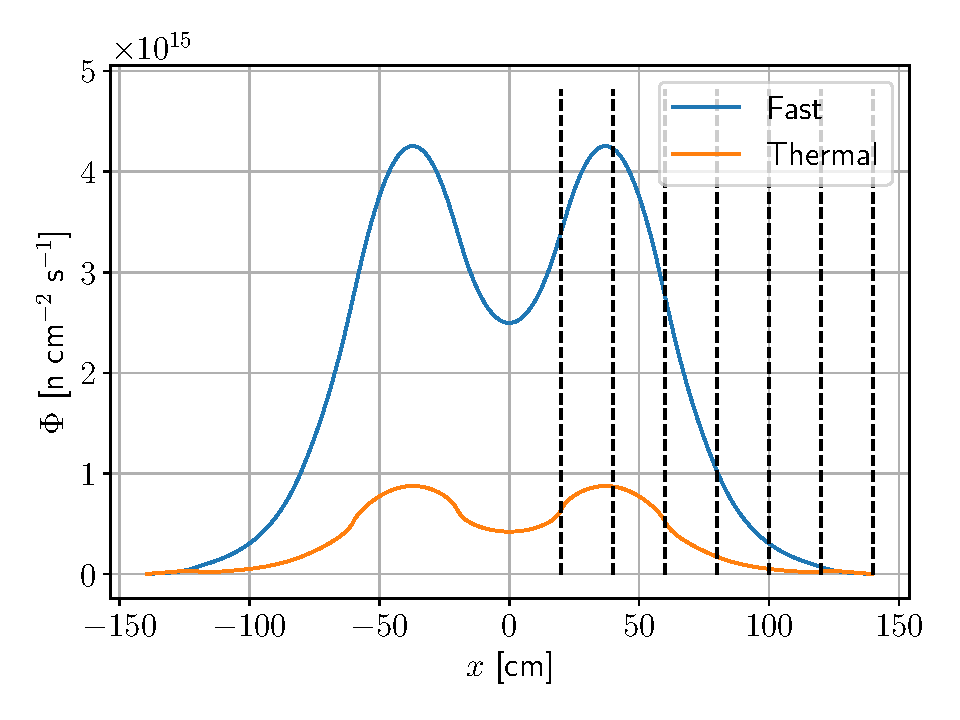
\includegraphics[width=10cm]{fig/Ex4_Flux_opti.pdf}
	\centering
	\caption{Normalized fast and thermal fluxes}
\end{figure}

\begin{figure}[H]
	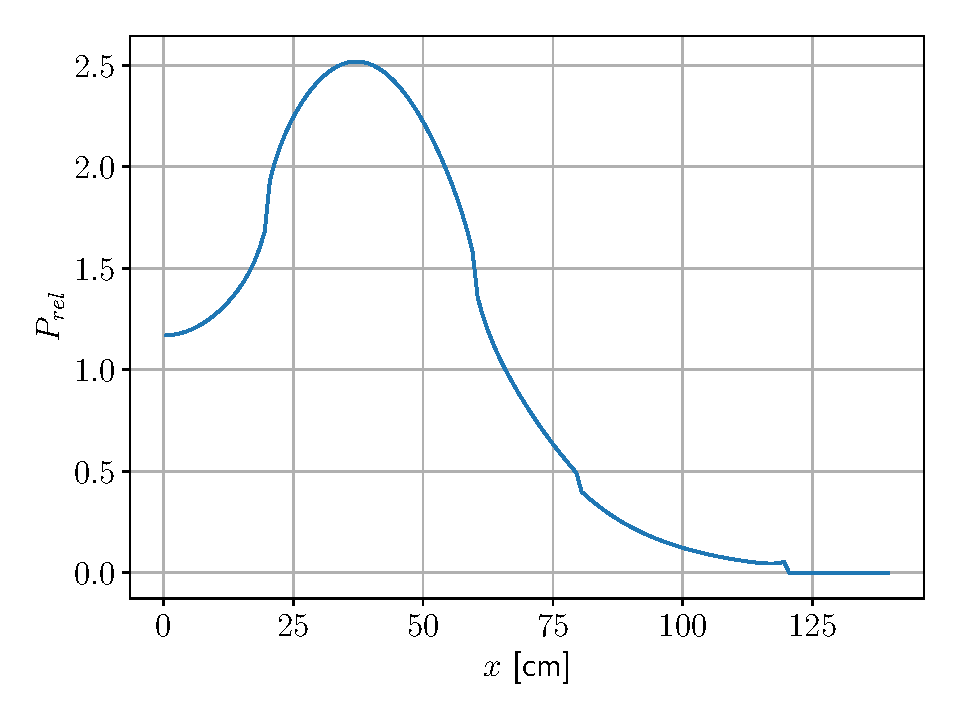
\includegraphics[width=10cm]{fig/Ex4_Power_opti.pdf}
	\centering
	\caption{Relative power distribution}
\end{figure}





% *******************************************************************************
% *** Exercice 5 ****************************************************************
% *******************************************************************************

\newpage
\section{Exercice \#5 - Fuel Evolution with exposure in a homogeneous media}



\end{document}
